\chapter{Trigonometry}

% !
\section{Basics - SOH CAH TOA}

\begin{tikzpicture}[scale=1.0]
  %define points A,B,C
  \tkzDefPoint(0,0){C}
  \tkzDefPoint(8,0){B}
  \tkzDefPoint(8,4){A}
  %label point A,B,C
  \tkzLabelPoints(B,C)
  \tkzLabelPoints[above](A)
  %draw triangleABC
  \tkzDrawPolygon[thick,fill=yellow!15](A,B,C)
  %marking right angles    
  \tkzMarkRightAngle(A,B,C)    
  %marking the angles
  \tkzFillAngle[fill=blue!20, opacity=0.5](B,C,A)
  \tkzLabelAngle[pos=1.25](B,C,A){$\theta$}
  \tkzMarkAngle(B,C,A)
  %label the sides
  \tkzLabelLine[pos=0.5,above, ](C,A){hypotenuse}
  \tkzLabelLine[pos=0.5,below, ](C,B){adjacent}
  \tkzDrawSegment[style=red, dim={opposite,15pt,midway,font=\normalsize, rotate=90}](A,B)
  %draw the points
  \tkzDrawPoints(A,B,C)
\end{tikzpicture}\\[18pt]

\begin{minipage}{0.5\textwidth}
  \begin{equation*}
    \sin \theta = \frac{\text{opposite}}{\text{hypotenuse}} = \frac{BA}{CA}
  \end{equation*}

  \begin{equation*}
    \cos \theta = \frac{\text{adjacent}}{\text{hypotenuse}} = \frac{CB}{CA}
  \end{equation*}

  \begin{equation*}
    \tan \theta = \frac{\text{opposite}}{\text{adjacent}} = \frac{BA}{CB}
  \end{equation*}
\vspace{0.5cm}
\end{minipage}
\begin{minipage}{0.5\textwidth}
  \begin{equation*}
    \csc \theta = \frac{1}{\sin \theta} = \frac{CA}{BA}
  \end{equation*}

  \begin{equation*}
    \sec \theta = \frac{1}{\cos \theta} = \frac{CA}{CB}
  \end{equation*}

  \begin{equation*}
    \cot \theta = \frac{1}{\tan \theta} = \frac{CB}{BA}
  \end{equation*}
\end{minipage}


% !
\section{General and Pythagorean Identities}

\begin{minipage}{0.4\textwidth}
  \textbf{General}
  \begin{equation*}
    \sec \theta = \frac{1}{\cos \theta}
  \end{equation*}

  \begin{equation*}
    \tan \theta = \frac{\sin \theta}{\cos \theta}
  \end{equation*}

  \begin{equation*}
    \cot \theta = \frac{1}{\tan \theta} = \frac{\cos \theta}{\sin \theta}
  \end{equation*}
\vspace{0.5cm}
\end{minipage}
\begin{minipage}{0.3\textwidth}
  \textbf{Pythagorean Identities}
  \begin{equation*}
    \sin^2 \theta + \cos^2 \theta = 1
  \end{equation*}

  \begin{equation*}
    \sec^2 \theta - \tan^2 \theta = 1
  \end{equation*}

  \begin{equation*}
    \csc^2 \theta - \cot^2 \theta = 1
  \end{equation*}
\end{minipage}


% !
\section{Unit Circle}

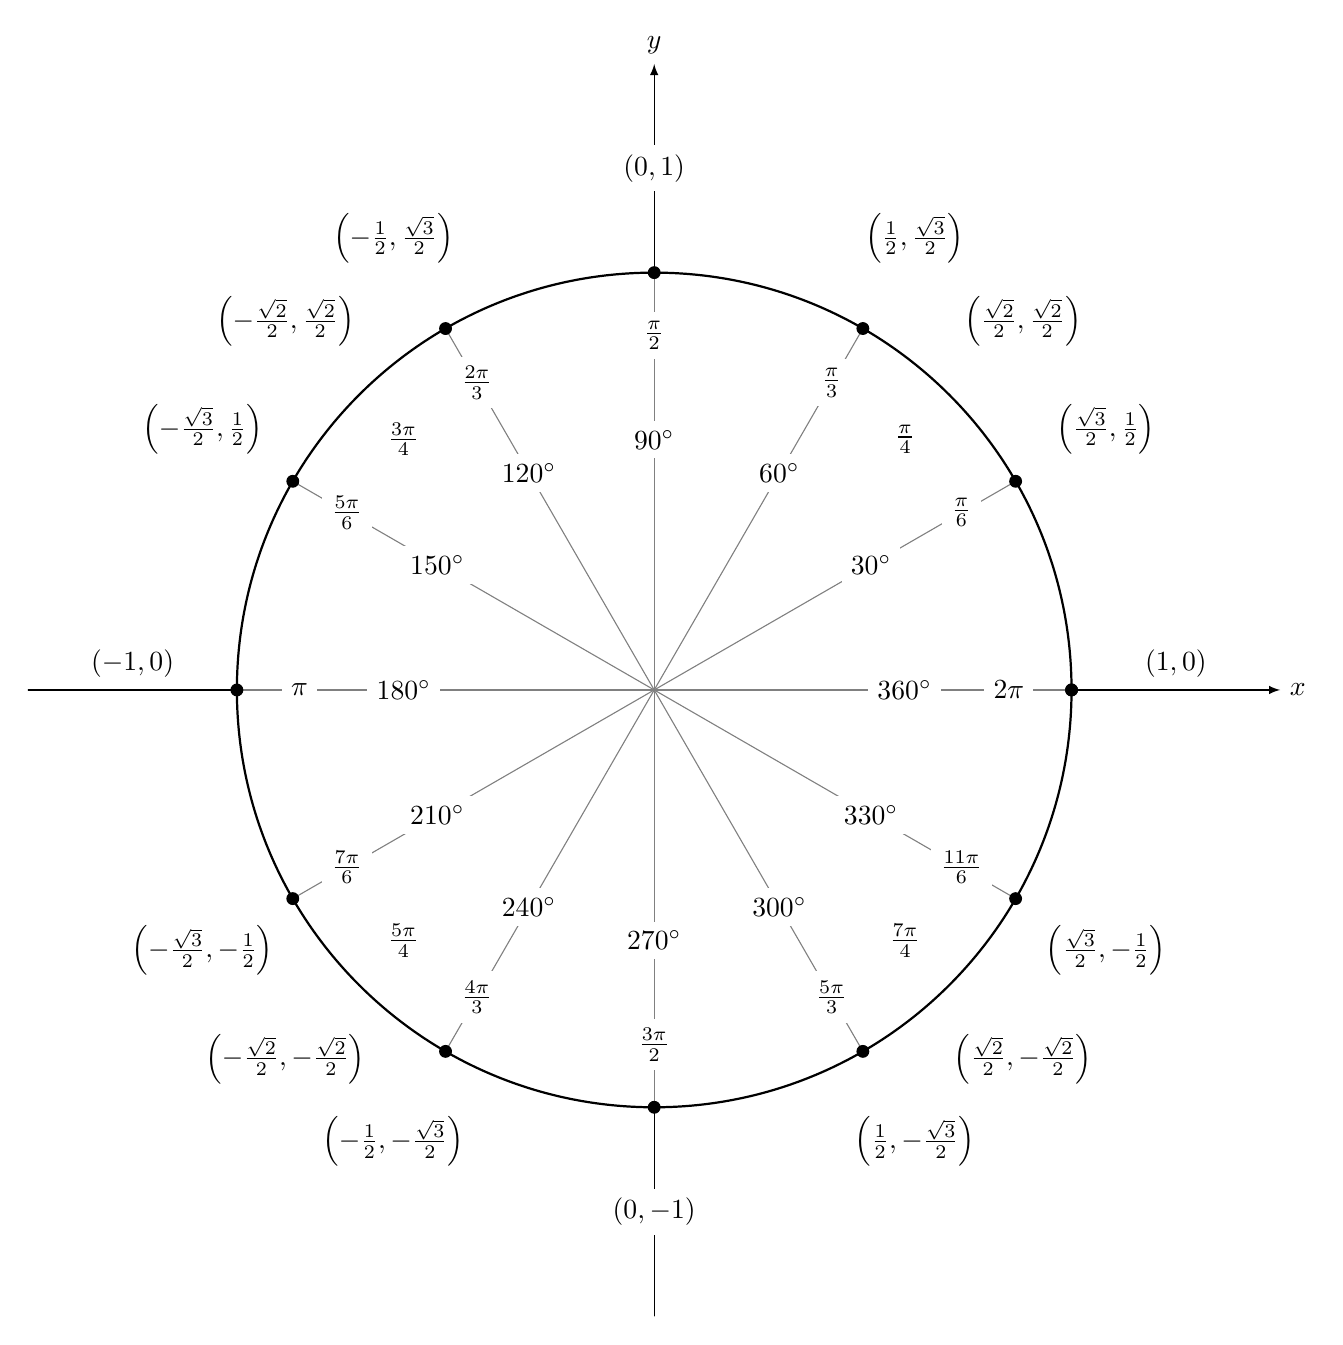
\begin{tikzpicture}[scale=5.3,cap=round,>=latex]
  % draw the coordinates
  \draw[->] (-1.5cm,0cm) -- (1.5cm,0cm) node[right,fill=white] {$x$};
  \draw[->] (0cm,-1.5cm) -- (0cm,1.5cm) node[above,fill=white] {$y$};

  % draw the unit circle
  \draw[thick] (0cm,0cm) circle(1cm);

  \foreach \x in {0,30,...,360} {
          % lines from center to point
          \draw[gray] (0cm,0cm) -- (\x:1cm);
          % dots at each point
          \filldraw[black] (\x:1cm) circle(0.4pt);
          % draw each angle in degrees
          \draw (\x:0.6cm) node[fill=white] {$\x^\circ$};
  }

  % draw each angle in radians
  \foreach \x/\xtext in {
      30/\frac{\pi}{6},
      45/\frac{\pi}{4},
      60/\frac{\pi}{3},
      90/\frac{\pi}{2},
      120/\frac{2\pi}{3},
      135/\frac{3\pi}{4},
      150/\frac{5\pi}{6},
      180/\pi,
      210/\frac{7\pi}{6},
      225/\frac{5\pi}{4},
      240/\frac{4\pi}{3},
      270/\frac{3\pi}{2},
      300/\frac{5\pi}{3},
      315/\frac{7\pi}{4},
      330/\frac{11\pi}{6},
      360/2\pi}
          \draw (\x:0.85cm) node[fill=white] {$\xtext$};

  \foreach \x/\xtext/\y in {
      % the coordinates for the first quadrant
      30/\frac{\sqrt{3}}{2}/\frac{1}{2},
      45/\frac{\sqrt{2}}{2}/\frac{\sqrt{2}}{2},
      60/\frac{1}{2}/\frac{\sqrt{3}}{2},
      % the coordinates for the second quadrant
      150/-\frac{\sqrt{3}}{2}/\frac{1}{2},
      135/-\frac{\sqrt{2}}{2}/\frac{\sqrt{2}}{2},
      120/-\frac{1}{2}/\frac{\sqrt{3}}{2},
      % the coordinates for the third quadrant
      210/-\frac{\sqrt{3}}{2}/-\frac{1}{2},
      225/-\frac{\sqrt{2}}{2}/-\frac{\sqrt{2}}{2},
      240/-\frac{1}{2}/-\frac{\sqrt{3}}{2},
      % the coordinates for the fourth quadrant
      330/\frac{\sqrt{3}}{2}/-\frac{1}{2},
      315/\frac{\sqrt{2}}{2}/-\frac{\sqrt{2}}{2},
      300/\frac{1}{2}/-\frac{\sqrt{3}}{2}}
          \draw (\x:1.25cm) node[fill=white] {$\left(\xtext,\y\right)$};

  % draw the horizontal and vertical coordinates
  % the placement is better this way
  \draw (-1.25cm,0cm) node[above=1pt] {$(-1,0)$}
  (1.25cm,0cm)  node[above=1pt] {$(1,0)$}
  (0cm,-1.25cm) node[fill=white] {$(0,-1)$}
  (0cm,1.25cm)  node[fill=white] {$(0,1)$};
\end{tikzpicture}


% !
\section{Half Angle Formulas}
\begin{equation*}
  \sin \left(\frac{A}{2}\right) = \pm \sqrt{\frac{1-\cos A}{2}}
\end{equation*}

\begin{equation*}
  \cos \left(\frac{A}{2}\right) = \pm \sqrt{\frac{1+\cos A}{2}}
\end{equation*}

\begin{equation*}
  \tan \left(\frac{A}{2}\right) = \pm \sqrt{\frac{1-\cos A}{1+ \cos A}}
  = \frac{\sin A}{1 + \cos A} = \frac{1 - \cos A}{\sin A}
\end{equation*}


% !
\section{Trig Addition and Subtraction Formulas}
\begin{minipage}{0.4\textwidth}
\begin{framed}
  \begin{equation*}
    \sin (A + B) = \sin A \cos B + \cos A \sin B
  \end{equation*}

  \begin{equation*}
    \sin (A - B) = \sin A \cos B - \cos A \sin B
  \end{equation*}

  \begin{equation*}
    \cos (A + B) = \cos A \cos B - \sin A \sin B
  \end{equation*}

  \begin{equation*}
    \cos (A - B) = \cos A \cos B + \sin A \sin B
  \end{equation*}

  \begin{equation*}
    \tan (A + B) = \frac{\tan A + \tan B}{1 - \tan A \tan B}
  \end{equation*}

  \begin{equation*}
    \tan (A - B) = \frac{\tan A - \tan B}{1 + \tan A \tan B}
  \end{equation*}
\vspace{0.5cm}
\end{framed}
\end{minipage}
\begin{minipage}{0.4\textwidth}
\begin{framed}
  Angle addition formulas express trigonometric functions of sums of angles
  A $\pm$ B in terms of functions of A and B. The fundamental formulas of angle 
  addition in trigonometry. 
\end{framed}
\end{minipage}


% !
\section{Double Angle Formulas}
\begin{minipage}{0.7\textwidth}
\begin{framed}
  Recalling the addition formula described below,
  \begin{equation*}
    \sin (A + B) = \sin A \cos B + \cos A \sin B
  \end{equation*}

  \begin{equation*}
    \cos (A + B) = \cos A \cos B - \sin A \sin B
  \end{equation*}

  \begin{equation*}
    \tan (A + B) = \frac{\tan A + \tan B}{1 - \tan A \tan B}
  \end{equation*}

  We consider what happens if we let B equal to A. then the first of these
  formulas becomes

  \begin{equation*}
    \sin (A + A) = \sin A \cos A + \cos A \sin A
  \end{equation*}

  so that

  \begin{equation*}
    \sin 2A = 2\sin A \cos A
  \end{equation*}

  If we do the same for the second equation

  \begin{equation*}
    \cos (A + A) = \cos A \cos A - \sin A \sin A
  \end{equation*}

  so that

  \begin{equation*}
    \cos 2A = \cos^2A - \sin^2A
  \end{equation*}

  Similarly

  \begin{equation*}
    \tan (A+A) = \frac{\tan A + \tan A}{1 - \tan A \tan A}
  \end{equation*}

  so that

  \begin{equation*}
    \tan (2A) = \frac{2\tan A}{1 - \tan^2A}
  \end{equation*}
\vspace{0.5cm}
\end{framed}
\end{minipage}

% !
\section{Power Reducing Formulas}
\begin{minipage}{0.7\textwidth}
\begin{framed}
  For $\sin^2\theta$:
  \begin{equation*}
    \cos 2\theta = \cos^2\theta - \sin^2\theta
  \end{equation*}

  \begin{equation*}
    \cos 2\theta = (1 - \sin^2\theta) - \sin^2 \theta
  \end{equation*}

  \begin{equation*}
    \cos 2\theta = 1 - 2 \sin^2\theta
  \end{equation*}

  \begin{equation*}
    \frac{2sin^2\theta}{2} = \frac{1-\cos 2\theta}{2}
  \end{equation*}

  \begin{equation*}
    \sin^2\theta = \frac{1-\cos 2\theta}{2}
  \end{equation*}

  For $\cos^2\theta$:
  \begin{equation*}
    \cos 2\theta = \cos^2\theta - \sin^2\theta
  \end{equation*}

  \begin{equation*}
    \cos 2\theta = \cos^2\theta - (1 - \cos^2\theta)
  \end{equation*}

  \begin{equation*}
    \cos 2\theta = \cos^2\theta - 1 + \cos^2\theta
  \end{equation*}

  \begin{equation*}
    \cos 2\theta = 2\cos^2\theta - 1 
  \end{equation*}

  \begin{equation*}
    \frac{\cos 2\theta+1}{2} = \frac{2\cos^2\theta}{2}
  \end{equation*}

  \begin{equation*}
    \cos^2\theta = \frac{\cos 2\theta + 1}{2}
  \end{equation*}

  For $\tan^2\theta:$
  \begin{equation*}
    \sin^2\theta + \cos^2\theta = 1
  \end{equation*}

  \begin{equation*}
    \frac{\sin^2\theta}{\cos^2\theta} + \frac{\cos^2\theta}{\cos^2\theta} = 
    \frac{1}{cos^2\theta}
  \end{equation*}

  \begin{equation*}
    \tan^2\theta + 1 = \sec^2\theta
  \end{equation*}

  \begin{equation*}
    \tan^2\theta = \sec^2\theta - 1
  \end{equation*}

\vspace{0.5cm}
\end{framed}
\end{minipage}


\section{Evaluating Inverse Trig}

\begin{framed}
  \noindent Evaluate on the range of
  \begin{equation*}
    \operatorname{arcsin} = -\frac{\pi}{2} \le R \le \frac{\pi}{2}
  \end{equation*}
\end{framed}

\begin{framed}
  \noindent Evaluate on the range of
  \begin{equation*}
    \operatorname{arctan} = -\frac{\pi}{2} < R < \frac{\pi}{2}
  \end{equation*}
\end{framed}

\begin{framed}
  \noindent Evaluate on the range of
  \begin{equation*}
    \operatorname{arccos} = 0 \le R \le \pi
  \end{equation*}
\end{framed}